\documentclass[11pt, a4paper]{article}

\usepackage[utf8]{inputenc}
\usepackage{authblk}
\usepackage{titlesec}


% Maths tools
\usepackage[tbtags]{amsmath}
\usepackage{amssymb}

% Margin
\usepackage[margin=2.8cm]{geometry}

% Line numbers
\usepackage{lineno}

% Spacing
\usepackage{setspace}
\doublespacing

% Enumeration
\usepackage{enumerate}% http://ctan.org/pkg/enumerate
\usepackage{enumitem}


% indentation
\setlength\parindent{10pt}
\setlength{\parskip}{5pt}

% Figures
\usepackage{graphicx}
\usepackage{caption}
\usepackage{subcaption}
\usepackage{epstopdf}
\usepackage{float}
\renewcommand{\thefigure}{\textbf{\arabic{figure}}}
\renewcommand{\figurename}{\textbf{Figure}}


%table
\usepackage{multirow}% http://ctan.org/pkg/multirow
\usepackage{hhline}
\usepackage[table]{xcolor}

\usepackage{authblk}


% References
\usepackage[round]{natbib}
\bibliographystyle{ecology_letters2.bst}

\usepackage{color, xcolor,soul}
%\definecolor{blau}{RGB}{168,221,181}
\definecolor{blau}{RGB}{236,226,240}
\soulregister\cite7
\soulregister\citenum7
\soulregister\citep7
\soulregister\citealt7
\soulregister\citealp7
\soulregister\citet7
\soulregister\ref7

% References and links
\PassOptionsToPackage{hyphens}{url}\usepackage[colorlinks=true,linkcolor=magenta, citecolor=magenta]{hyperref}

%Margin notes
\usepackage{marginnote}
% Foot note distance with text
\usepackage[symbol]{footmisc}
\renewcommand{\thefootnote}{\fnsymbol{footnote}}
\setlength{\skip\footins}{0.75cm}

%Define colour
\DeclareRobustCommand{\hlc}[1]{{\sethlcolor{blau}\hl{#1}}}

%subsubsection format
\titleformat*{\subsubsection}{\large\it}

\makeatletter
\renewcommand\AB@affilsepx{; \protect\Affilfont}
\makeatother

%Title paper
\title{\vspace{-1cm}
Model linearity breeds contempt: using Bayesian non-linear models to uncover general biogeographical patterns}
% Model familiarity breeds contempt: simple models to compare properties of species' distributions
% Model simplicity breeds contempt: simple models to compare properties of species' distributions
% Model complexity breeds contempt: using non-linear models to compare basic properties of species' distributions
\author[1,*]{\normalsize Bernat Bramon Mora}
\author[1]{\normalsize Jake M.\ Alexander}
\affil[1]{\footnotesize Institute of Integrative Biology, ETH Zürich, Zürich, Switzerland}
\affil[*]{\footnotesize  bernat.bramon@gmail.com}

\renewcommand\Authands{ and }
\date{}

\begin{document}
\maketitle
\linenumbers

\section*{Abstract}

Species' distribution models have emerged as one of the most influential methodological advances in ecology and biogeography of the last decades. Useful to understand how populations of species will change along environmental gradients, they have become ecologists' compass to predict the effects of global climate change. That said, uncovering the mechanisms shaping species' realized niches has been one of the main driving forces behind the development of these models. That is, recent efforts have been often focused on understanding which biotic and abiotic factors are good predictors of species' niches---with an increasing effort placed in improving the predictive power of the statistical models. However, we still lack a general understanding of the shape of species' distributions, and much less is known about how these distributions compare to each other across gradients. Here, we use a set of Bayesian non-linear models to uncover the shape of species' realized niches. These models account for all prior knowledge we have regarding their shape, including expert knowledge on species' environmental preferences and physiology. With this approach, we are able to shed light on the true shape of empirical species' distributions. Moreover, they allow us to tackle long-standing hypothesis regarding general biogeographical patterns. In particular, we found conclusive evidence of the relationship between several properties of distributions, including the link between species' range size and elevation and their skewness along gradients. Finally, we are able to shed light on the extent to which some aspects of the shape of observed realized niches---such as kurtosis and skewness of the distributions---could be intrinsic properties of species. Overall, our approach offers a useful statistical framework to understand the shape of species' distributions, and our results provide an unprecedented perspective of the way systems of many species are distributed along environmental gradients.

\section*{Introduction}

%Consider testing tails of distribution? I would use the Cauchy or generalized normal distribution for heavy tail distribution without skewness; and I would use an exponentially modified Gaussian distribution with heavy tails for a skew distribution with heavy tails. 
% Option (1) for a long-tail distribution: Generalized normal distribution. We model it such that shape parameter beta can go from 1 to 8
% Option (2) for a long-tail distribution: Student's t-distribution. In this case, we would need to define the shape parameter so that it is larger than 2 (otherwise, we would have undefined variance)
% Option (1) for a long-tail skewed distribution. The exponentially modified Gaussian distribution has potential, but I am not sure I can fit a parameter that goes from like lambda if I want the skewness in either side.
% Option (2) for a long-tail skewed distribution. Version 2 of the Generalized normal distribution. The problem here is that this function has a few discontinuities, which means that one needs to use a step function. I believe this to be quite problematic in Stan...
% Option (3) for a long-tail skewed distribution. Skewed student-t distribution. This seems to be complex but quite what I need. It will be hard to fit but seems quite promising. See:
%https://www.tandfonline.com/doi/abs/10.1080/01621459.1998.10474117
%https://hess.copernicus.org/preprints/hess-2015-24/
%https://agupubs.onlinelibrary.wiley.com/doi/epdf/10.1029/2009WR008933


One of the central goals of ecology is to understand the ways species are distributed across space and time (ref). Over the last two decades, ecologists have developed multiple distribution models to try to untangle the factors that play a role in defining such distributions \citep{guisanPredictiveHabitatDistribution2000}. These models estimate species' realized niches using several covariates, including environmental variables \citep{guisanPredictingSpeciesDistribution2005}, species ecological traits' \citep{pollockRoleFunctionalTraits2012} and phylogenetic relations \citep{ivesGeneralizedLinearMixed2011}. More recently, some of the focus have shifted towards approaches that estimate and account for biotic factors, such as competitive or facilitative relationships between species \citep{ovaskainenHowMakeMore2017}. The idea is that by untangling the ways in which such biotic and abiotic factors shape species' distributions, we can gain a mechanistic understanding on how ecological communities are established and change over time. However, while these factors can increase the predictive performance of some of the models \citep{norbergComprehensiveEvaluationPredictive2019}, the interpretation of the corresponding parameter estimates has been recently questioned \citep{harrisInferringSpeciesInteractions2016, thurmanTestingLinkSpecies2019, poggiatoInterpretationsJointModeling2021}. This was best illustrated by \citet{blanchetCooccurrenceNotEvidence2020}, who used basic statistical arguments to highlight the artefactual nature of the link between co-occurrence and species' ecological interactions drawn by some distribution models.
% Other references for biotic interaction=bad: dormannBioticInteractionsSpecies2018

The value of gaining a mechanistic understanding of species' distributions is unquestionable (ref), with several studies highlighting the importance of factors such as biotic interactions and dispersal ability in setting species' range limits \citep{wiszRoleBioticInteractions2013, pollockUnderstandingCooccurrenceModelling2014, neuschulzBioticInteractionsSeed2018}. That said, a lot can be learned from taking a phenomenological approach, focussing instead on the description of basic properties of species' realized niches. For example, the study of species' range sizes along environmental gradients can reveal general biodiversity patterns that are crucial from a conservation and management perspective \citep{stevensElevationalGradientAltitudinal1992}. Differences in species' responses to the environment could shed light on how climatic processes and historical contingencies have shaped their distributions \citep{rohdeLatitudinalGradientsSpecies1992, more in Rapoport}. Other properties, such as the skewness of species' distributions, can also reveal general underlying processes regarding species' physiological tolerance to different environmental conditions \citep{kaufmanDiversityNewWorld1995}. More generally, understanding the shape of species' realized niches and the extend to which these vary across species is a crucial issue in ecology and biogeography (ref); however, we do not have an effective way to parsimoniously compare the realized niches of many species. Indeed, there is no general agreement on the shape of species' distributions (ref).

Many ecological textbooks \citep{krebsEcologyExperimentalAnalysis1972} assume the shape of species distributions to be unimodal and symmetric, but some have warned that empirical distributions can take many different forms \citep{austinModelsAnalysisSpecies1987, austinSpatialPredictionSpecies2002}. In practice, distribution frameworks often use logistic regressions with a linear relationship between covariates (but see \citealt{review} and \citealt{good example}). This is useful because it simplifies the optimization process, but it comes with some statistical shortcomings. First and foremost, such response curve and the linear relationship between covariates often comes with a set of implicit mathematical constrains that might not be biologically justified. From a purely statistical perspective, if all that we are willing to assume is that species occupy finite geographic ranges---i.e.~their probability distributions have finite variance---the most conservative statistical approach is to model these as a Gaussian distributions \citep{frankCommonPatternsNature2009}. Other factors might then condition species distributions to showcase heavy-tails or a skewed shapes, revealing interesting ecological processes shaping biodiversity patterns \citep{austinNonlinearSpeciesResponse1976, minchinEvaluationRelativeRobustness1987}. The starting point, nevertheless, should be the one that makes the fewest assumptions (i.e.~the maximum entropy distribution; \citealt{frankCommonPatternsNature2009}), and every new shape will imply a hypotheses on how communities are distributed \citep{damenSpatialPredictionsCommunity2017}. Second, the aforementioned structural constrains also limit our ability to include any prior information to our parameter estimates. Observations on species' geographic variation and optimal climatic conditions have long been documented, with extensive databases compiled by botanists and field ecologists documenting basic knowledge on species' realized niches (e.g.~\citealt{landoltFloraIndicativaOkologische2010}). That said, this information is rarely accounted for in most modelling approaches, potentially because there is not a straightforward way to feed this information into the parameters of a linear model (\citealt{scherrerEcologicalIndicatorValues2019}; but see \citealt{terbraakWeightedAveragingLogistic1986, ovaskainenHowMakeMore2017}). Finally, and perhaps most importantly, a direct biological interpretation of parameter estimates in linear models becomes increasingly difficult as one moves from unimodal and symmetric distributions \citep{terbraakWeightedAveragingLogistic1986, jamilGeneralizedLinearMixed2013} to skewed distributions \citep{huismanHierarchicalSetModels1993}, making the tests of hypothesis on global biodiversity patterns particularly challenging. For example, \citet{huismanHierarchicalSetModels1993} proposed several non-linear models to characterize several features of species' response curves; however, species' environmental indicator values, range size or distribution skewness are difficult to understand altogether following these model structures.

%This is rarely the starting point in most statistical frameworks that study general biodiversity patterns (but see ref), choosing to use instead Gaussian-logit response curves (refs).
%\citet{} showed that bell curves are not universal response curves in vegetation data, with distributions often presenting skewed responses, and some modelling techniques try to account for this asymmetry in species distributions.

The field of ecology has quickly moved towards mechanistic and process-based approaches to understand species' distributions \citep{wartonManyVariablesJoint2015}. This has resulted in a plethora of models accounting for several biotic and abiotic factors into the predictions of species co-occurrence. Here, we instead rethink traditional modelling approaches and develop a conceptually simple---and yet statistical and computationally complex---statistical framework to revisit some classic hypothesis in ecology and biogeoraphy. In particular, we develop a Bayesian hierarchical model that accounts for all prior information that we have regarding the distribution of alpine plant species along an elevation gradient in the Swiss Alps, including expert knowledge on species environmental indicator values, range sizes, and plant physiology. We start by considering species' response curves as Gaussian distributed, and then we adapt our model to allow for skewed and long-tailed distributions. Using this statistical framework, we are able to compare the basic properties of the realized niches of multiple species, testing for the existence of general biogeographical patterns. First, we test for the Rapopor's rule, which predicts a positive relationship between range size and elevation \citep{stevensElevationalGradientAltitudinal1992}. While this pattern has been largely studied for multiple systems and across gradients \citep{mccainElevationalRapoportRule2013}; contrasting evidence suggests this rule not to be pervasive across species \citep{ribasRapoportEffectWidespread2006, bhattaraiCanRapoportRule2006, mccainElevationalRapoportRule2013}. Our results not only allow us to properly test the existence of this geographical pattern, but they also showcase variation in how different types of species, such as native or neophytes, might respond to an environmental gradient. Second, we study whether or not species' distributions show steeper declines towards stressful conditions, testing the so-called abiotic stress limitation hypothesis (ref). \citet{normandImportanceAbioticStress2009} tested this for vegetation data using \citeauthor{huismanHierarchicalSetModels1993}'s statistical models for several independent species, finding no clear support for such a hypothesis. Our results are able to shed light on this geographical pattern as well as to highlight the degree to which different species will showcase different levels of decline towards stressful conditions. Specifically, we are able to link plant physiological traits to the skewness of their distributions. Overall, we use models that are solely constrained by the empirical information that we truly have regarding our system, relaxing as much as possible the structural constrains of the statistical framework. Using these models, we are able uncover the approximate shape of empirical plant distributions and answer fundamental questions regarding the way systems of many species are distributed along environmental gradients.


%%%%%%%%%%%%%%%%%%%%%%%FINAL



% To decide among modelling approaches, we first need to agree on what we know about the system. We know that species occupy a geographic range; therefore, we know that their distributions have finite variance. Indeed, observations on species' geographic variation and optimal climatic conditions have been long documented, with extensive databases compiled by botanists and field ecologists documenting basic knowledge on species' distributions. One could point out that we also know that many other factors might influence species' presence/absence---e.g. the influence of the aforementioned biotic interactions among species. However, we do not necessarily have an intuition of how exactly these factors will influence the shape of species' distributions. Therefore, if all we truly knew about a species' distribution was that they have finite variance, the most conservative assumption and the safest bet---i.e. the one with the largest entropy---is that such distribution is a Gaussian.


%The strength of climate as a range limiting factor will becrucial for the extent to which species will retract from theirsouthern range margins and expand northwards under global warming. occurrence of a species along an environmentalgradient may primarily be limited by its physiological tolerancetowards the abiotically more stressful conditions, while otherfactors, such as biotic interactions, may assume a greater roletowards less stressful conditions (Connell, 1961; Austin, 1990;Brown  et al. , 1996); hereafter referred to as the asymmetricabiotic stress limitation (AASL) hypothesis.

%abiotic stress is generally thought to increasetowards high latitudes and altitudes and to decrease in importancetowards the equatorial lowlands, where biotic interactions havebeen argued to increase in importance (Dobzhansky, 1950;Kaufman, 1995). Accordingly, a geographical prediction of theAASL hypothesis is that abiotic stress may be most importantin upper-latitudinal and upper-altitudinal range boundaries(MacArthur, 1972; Brown  et al. , 1996), but this has received littlestudy. Loehle (1998) suggested that the northern and southernrange limits of North American tree species are determined bycold tolerance and competitive ability, respectively. Similarly,abiotic stress appears to determine the upper-altitudinal rangelimit for some mountainous plant species, while biotic interactionsmay determine the lower limit (Guisan  et al ., 1998; Bruelheide &Scheidel, 1999; Vetaas, 2002). A second aspect of the AASL hypothesis proposes that theshape of species response curves vary along an environmentalgradient: species that occur under the physiologically moststressful conditions show skewed responses with a steep declinetowards the stressful conditions, while species that occur underless stressful conditions show symmetric responses (Austin,1990; also cf. Austin  et al ., 1994; Austin & Gaywood, 1994;Rydgren  et al. , 2003). In line with this, Kaufman (1995) suggeststhat the degree to which a species’ poleward range boundary islimited by abiotic stress increases the further north the species isdistributed. Analogously, we expect increasing stress limitationwith increasing elevation

% Guisan found no evidence of that. 
% No support for Kaufman’s (1995) geographical prediction ofthe AASL hypothesis,

 %There is not an easy way to untangle the true shape of species' distributions, as this shape is likely to showcase idiosyncrasies at the species level and across systems. The aim of this work, it is not to answer these questions nor to provide a general approach that accommodates such idiosyncrasies. Instead, we want to use a model that is solely constrained by the empirical information that we truly have regarding a particular system, relaxing as much as possible the structural constrains of the statistical framework. Then, we want to use this model to answer basic aspects regarding the way systems of many species are distributed along an environmental gradient. 


%%%%%%%%%%%%%%% KEY PAPERS AND IDEAS REGARDING HYPOTHESES #################
% EXPLAIN WHY KNOWING THIS BASIC INFORMATION IS IMPORTANT 
% WHY DO YOU CARE
% ABUNDANCE CENTER HYPOTHESIS IDEA
% HOW STEEP THE EDGES ARE RAPIDLY EXPANDING
% species’ thermal tolerance breadths 
% https://eco.confex.com/eco/2020/meetingapp.cgi/Paper/86915
% https://advances.sciencemag.org/content/5/11/eaaz0414
% https://onlinelibrary.wiley.com/doi/full/10.1111/j.1466-8238.2009.00451.x
% https://royalsocietypublishing.org/doi/10.1098/rspb.2010.1295



%%%%%%%%%%%%%%   Species thermal tolerance breadths   %%%%%%%%%%%%%%%%%%%%%
% Species' thermal tolerance increases with latitude (elevation). The asymmetricabiotic stress limitation (AASL) hypothesis
% - mostly macroecological patterns. What about along elevational gradient?
% - Taxonomic scope often restricted. What about plants?
% - upper and lower thermal tolerance data are not always sampled from the same species. Bayes solve the problem?


%Comparisons of the predictive performance of such models are also extensive (ref), untangling the modelling approaches that better capture variation in species' distributions. 

% People comparing performance: Wilkinson, D. P., N. Golding, G. Guillera‐Arroita, R. Tingley, and M. A. McCarthy. 2019. A comparison of joint species distribution models for presence–absence data. Methods in Ecology and Evolution 10:198–211; A comprehensive evaluation of predictive performance of 33 species distribution models at species and community levels

%The last two decades have seen a proliferation of species distribution models (SDMs) addressing the challenge of predicting the occurrences of individual species (Guisan and Zimmermann 2000, Guisan and Thuiller 2005, Elith et al. 2006, Leathwick et al. 2006, Zimmermann et al. 2010). Methodological advances in multiple‐species distribution modeling have lagged behind, but are recently experiencing a rapid expansion (Leathwick et al. 2006, Dunstan et al. 2011, Guisan and Rahbek 2011, Warton et al. 2015, Wilkinson et al. 2019). Many previous studies (Table 1) have compared the predictive performance of SDMs for single‐species analyses (Moisen and Frescino 2002, Thuiller et al. 2003, Elith et al. 2006, Leathwick et al. 2006, Elith and Graham 2009, Guisan and Rahbek 2011). Some studies have compared single‐species and multi‐species distribution models (Araújo and Luoto 2007, Heikkinen et al. 2007, Baselga and Araújo 2009, 2010, Elith and Leathwick 2009, Chapman and Purse 2011, Bonthoux et al. 2013, Madon et al. 2013, Maguire et al. 2016, Harris et al. 2018), while a few have examined the performance of alternative multiple species modeling approaches (Baselga and Araújo 2010, Madon et al. 2013, Wilkinson et al. 2019). 

%Overall, these methodological advances have provided with crucial ecological insights into the factors shaping species' distributions (ref); however, they have also faced some criticism as a result of the... For example, ...
%
%The use of species distribution models has grown a lot. These models try to estimate species' realized niches using several covariates, including environmental variables (ref), species ecological traits' (ref) and phylogenetic relations (ref). Recent work on these modelling approaches has increasingly focused on estimating (ref) and accounting for (ref) biotic factors, such as competitive or facilitative relationships. The idea is that by understanding how all such factors shape species' distribution we will gain a mechanistic understanding on how these distributions are established and change over time. Unfortunately, while some of this approaches will certainly increase the predictive performance of distribution models (ref), the nature of some of the estimates have been shown to theoretically have some mishaps (ref).

%Ecology has been described as the scientific understanding of factors determining the abundance and distribution of species (Smith 1966; Begon et al. 1986). This understanding can hardly be achieved by studying species one by one since their abundances and distributions depend not only on their indi- vidual responses to the abiotic environment, but also on their interactions (Wisz et al. 2013). Thus, a key aim in modern community ecology is to gain an integrative understanding of how biotic and abiotic factors mould local species pools at different spatiotemporal scales. Community ecology began as a descriptive science in which communities were classified based on the identities and sizes of local species pools (e.g. Clements 1936; Elton 1966). Mod- ern community ecology is progressing from the description of patterns towards a mechanistic perspective, which seeks to understand the processes determining the identities and abundances of the species from local to global spatiotemporal scales (Agrawal et al. 2007; Logue et al. 2011). During the last few decades, experimental ecologist have used observations and experiments to assess the relative influences of stochastic- ity, competition and niche differentiation (see Logue et al. 2011), theoretical ecologists have developed models for pre- dicting community dynamics (e.g. Tilman 1990, 2004; Holt et al. 1994; Bolker et al. 2003; Leibold et al. 2004; Holyoak et al. 2005), and statistical ecologists have developed metrics for assessing compositional changes among local communities (e.g. Gauch 1982; ter Braak & Prentice 1988; Legendre & Legendre 2012).



%\citet{austin2002spatial} writes "\textit{there are three major components in any framework for statistical modelling in plant ecology. There needs to be an ecological model, a data model, and a statistical model. The ecological model consists of the ecological knowledge and theory to be used or tested in the study. The data model consists of the decisions made regarding how the data are collected and how the data will be measured or estimated. The statistical model involves the choice of statistical method, error function and significance tests. Each model interacts in both obvious and subtle ways with the other models to determine the success of any statistical modelling exercise.}" While a lot of work has been developed for all three components outlined by \citet{austin2002spatial}, increasing emphasis has been put into advancing the data and statistical models. Indeed,


 
\section*{Methods}
\subsection*{Empirical data}
We studied the distribution of alpine plant communities along an elevation gradient. To do so, we combined two different datasets: i) one describing the co-occurrence of species across multiple open grasslands in the Swiss Alps, and ii) an extensive floristic database containing environmental and physiological traits for all vegetation across Switzerland \citep{landoltFloraIndicativaOkologische2010}. 

\subsubsection*{Distribution data}
We used data describing the distribution of 798 species across 912 sites covering most of the mountain region of the Western Alps in the Canton de Vaud (Switzerland; \citealt{scherrerEcologicalIndicatorValues2019}). Each of these sites is a $8\times 8\,\text{m}$ plot placed somewhere along an elevation range from $375\,\text{m}$ to $3210\,\text{m}$. In all sites, presence/absence data as well as Braun-Blanquet abundance-dominance classes were recorded for all species. Additionally, we used meteorological data provided by \citet{scherrerEcologicalIndicatorValues2019}, containing multiple variables characterizing the climate in each site at high spatial resolution ($25\,\text{m}$). This dataset was compiled based on 30 years (1961–1990) of records from national weather stations. Since most of the data is highly correlated, we calculated the main axes of variation of the following scaled variables: daily minimum, maximum and average temperature; sum of growing degree-days above $5^{\circ}\text{C}$; mean temperature of wettest quarter; annual precipitation, precipitation seasonality, and precipitation of driest quarter (see Supplementary Methods; Supplementary Fig. 1). %Missing TabsY

\subsubsection*{Floristic data}
To complement the aforementioned distribution data, we used a floristic database of most vegetation across Switzerland. This database was build based on expert knowledge and field experience of botanists and ecologists, and contains information regarding species' environmental preferences and physiological traits. Species' environmental preferences in this database can be used to inform distribution models---e.g.~as an informative prior in a Bayesian framework. These are characterized following the ecological indicator values developed by \citet{landoltFloraIndicativaOkologische2010}, providing both an estimate of the average conditions in which a species can be found as well as a broad description of their range of variation. These values are provided for a range of 10 climatic variables, including temperature, continentality, light conditions, as well as moisture, acidity and nutrient content of the soil (see a full list and description of the ecological indicators in the Supplementary Table 1; \citealt{landoltFloraIndicativaOkologische2010}). On the other hand, the information regarding species' physiological traits represents general descriptions of species' growth and life strategies---examples include their growth forms, nature of the storage organs, dispersal ability and pollinator agents. In total, we identify more than $120$ binary traits that characterize the physiology of species (see a full list and description of the ecological indicators in the Supplementary Table 1; \citealt{landoltFloraIndicativaOkologische2010}). Finally, and in addition to species' environmental preferences and physiological traits, the floristic data also contains information on species types (e.g.~identifying those species that are neophytes)---and change tendency (e.g.~indicating species that have shown decline or increase in their populations over the recent decades). We describe this information in more detail in the Supplementary Table 1.

%we independently consider those traits that describe growth and life strategies of the plants---examples include their growth forms, nature of the storage organs, dispersal ability and pollinator agents. In total, we identify $\sim120$ binary traits that characterize the physiology of species.

%comprising a total of 10 environmental indicator values with 10 types of associations for each of them (i.e. the $r$ associations defined above). Finally, we additionally independently consider species' range of variations for the such indicator values, also defining 10 `traits' with 3 types of associations (I need to see if I can added these to the analyses above).

%In this study we used the ecological indicator values (EIVs) first developed by Landolt17 and later extended by Landolt et al.19. Landolt’s EIVs are largely similar to the more renown ones proposed by Ellenberg et al.18, but specifically adapted to the flora and environmental conditions of Switzerland. There are a large number of EIVs (for details see Landolt et al.19), but in this study we focused on six of the most commonly used, namely: T for temperature;, M for soil moisture/water availability;, L for light;, K for continentality;, R for soil pH; and N for soil nutrients.
%Based on 30 years (1961–1990) of meteorological data from national weather stations, fourteen climatic variables (Table S5) were calculated according to the method described in Zimmermann & Kienast44 and Zimmerman et al.55. A digital elevation model (DEM) was used to spatially interpolate the climatic data and to create topographic variables (Table S5). Additionally, we used a soil pH map based on Buri et al.43. All environmental data had a spatial resolution of 25 m, a resolution similar to the areas used to calculate the ecological indicator values (EIV; see below). This allowed a straightforward comparison of different sets of predictors composed from environmental variables and EIVs.

%In this study we used the ecological indicator values (EIVs) first developed by Landolt17 and later extended by Landolt et al.19. Landolt’s EIVs are largely similar to the more renown ones proposed by Ellenberg et al.18, but specifically adapted to the flora and environmental conditions of Switzerland. There are a large number of EIVs (for details see Landolt et al.19), but in this study we focused on six of the most commonly used, namely: T for temperature;, M for soil moisture/water availability;, L for light;, K for continentality;, R for soil pH; and N for soil nutrients.

\subsection*{Baseline model}
There is a long list of model structures well suited to characterize species' distributions (see \citealt{norbergComprehensiveEvaluationPredictive2019}). As a baseline model, however, we were interested in a hierarchical model that does not make any assumptions regarding the shape of the distributions, and yet explicitly incorporates all information that we have regarding plant's environmental preferences. More specifically, we wanted to account for the climatic indicator values and range of variation registered in the floristic database for all plants in our dataset. These two values provide basic information regarding plant's optimal environmental conditions and width of their distributions.

\subsubsection*{Response curve}
To choose an appropriate response curve, we first need to agree on what we truly know about the system. Given the prior information that we have about the system, we know that species occupy specific geographic ranges; therefore, we know that their distributions have finite variance. While we could also assume that many other factors might influence species' presence in a given site---e.g.~the biotic interactions among specie in the site---we do not necessarily have an \textit{a priori} expectation of how exactly these factors will influence the shape of species' distributions. Therefore, for this baseline model, if all that we are willing to assume about species' realized niches is that these have finite variance, the most conservative assumption and the safest bet---i.e.~the one with the largest entropy---is that they follow a Gaussian distribution. That is, given the presence/absence or abundance $y_{ij}$ of any species $i$ in any given site $j$, and an environmental variable $x_{j}$, we define can species' responses to the environment as
\begin{equation}
\begin{split}
y_{ij} & \sim F\left(p_{ij}\right) \\
\text{log}\left(p_{ij}\right) & = -\alpha_{i} - \gamma_{i} \left(x_{j}-\beta_{i}\right)^2 ,
\end{split}
\label{eq:baseline-response}
\end{equation}
where $F$ is the likelihood function, and $\alpha_i$, $\beta_i^k$, and $\gamma_i$ describe amplitude of the probability $p_{ij}$, species' average climatic suitability and range of variation along the an environmental gradient, respectively. Notice that $F$ characterizes a Binomial distribution when considering binary data, and it characterizes an ordered categorical likelihood function when we consider Braun-Blanquet abundance-dominance classes as response variables (see the full description of both models in the Supplementary Methods). For the sake of simplicity, we use only one environmental variable to characterize species' probability distribution. That said, this model can easily be generalized to account for multiple predictors (see Supplementary Methods).

\subsubsection*{Model priors}
The model structure described above allows us to explicitly incorporate all prior knowledge that we have regarding species' distributions contained in the floristic database. To do so, we define the prior distributions for the parameters in model (\ref{eq:baseline-response}) as:
\begin{equation} 
\begin{split}
\beta_{i}  & \sim \text{MVNormal}\left(\hat{\beta}, \Sigma^{\beta}\right)\\
\text{log}(\gamma_{i})  & \sim \text{MVNormal}\left(\hat{\gamma}, \Sigma^{\gamma}\right)\\
\text{log}(\alpha_{i}) & \sim \text{Normal}\left(\hat{\alpha}, \sigma_{\alpha}\right)\\
\hat{\beta}, 
\hat{\gamma}, 
\hat{\alpha}  & \sim \text{Normal}\left(0,1\right)\\
\sigma_{\alpha}  & \sim \text{Exponential}\left(1\right)
\end{split}
\label{eq:baseline-priors}
\end{equation} 
where parameters $\gamma_i$ and $\beta_i$ are expressed as multivariate normal distributions---i.e.~Gaussian processes---such that $\Sigma^{\beta}$ and $\Sigma^{\gamma}$ are variance-covariance matrices describing species' similarity in terms of their average climatic suitability and range of variation along the different environmental gradients, respectively. We define these variance-covariance matrices as follows:
\begin{equation} 
\Sigma_{ij} = \eta\,\text{exp}\left(-\rho {D_{ij}}^2\right) + \delta_{ij} \sigma ,
\label{eq:covariance-baseline}
\end{equation}
where $\Sigma_{ij}$ characterizes the covariance between any pair of species $i$ and $j$, and $\delta_{ij}$ is the Kronecker delta. Notice that such a covariance structure declines exponentially with the square of a distance matrix $D_{ij}$, which characterize differences between species computed using our prior information. In the floristic database, this information is represented by the set of ordinal traits specified for the different species. While there are many different ways to turn ordinal data into distance matrices, we choose to use a mixed-membership stochastic block model because it allows us to deal with cases of missing data (see Supplementary Methods for extended details; \citealt{godoy-loriteAccurateScalableSocial2016}). In each covariance matrix, the hyperparameter $\rho$ determines the rate of decline of the covariance between any two species, and $\eta$ defines its maximum value. The hyperparameter $\sigma$ describes the additional covariance between the different observations for any given species. For all these hyperparameters, we choose weekly informative priors such that $\sigma , \eta \sim \text{Exponential}\left(1\right)$ and $\rho\sim \text{Exponential}\left(0.5\right)$.

\subsubsection*{Alternative variance-covariance structures}
The model structure defined above allows us to test how different sources of information characterize each of the different parameters. Specifically, we can do this by modifying Eq.~(\ref{eq:covariance-baseline}). For example, imagine that we have multiple matrices $D^k$ characterizing species' differences along different axis of variation---e.g.~two matrices characterizing physiological and environmental traits. One can modify Eq.~(\ref{eq:covariance-baseline}) for a particular parameter---e.g.~$\beta_{i}$---such that
\begin{equation} 
\Sigma_{ij} = \eta\,\text{exp}\left(-\sum_k\rho_{k} {D^{k}_{ij}}^2\right) + \delta_{ij} \sigma ,
\label{eq:covariance-complex}
\end{equation}
where now $\rho_{k}$ are separate relevance hyperparameters for each distance matrix in the total variance of $\beta_i$.

\subsubsection*{Sampling the posterior}
We generated the posterior samples for the Bayesian models with the Hamiltonian Monte Carlo algorithm implementation provided by the R package `rstan' to \citep{standevelopentteamRStanInterfaceStan2021}. Sampling models like the ones described above can be computationally very expensive. This is especially true when using ordered categorical likelihood functions (see \citealt{standevelopmentteamStanModelingLanguage2021}). Therefore, we focus on those species for which we have at least 20 occurrences when modelling binary data, which corresponds to the majority of the results of this work. When using ordinal data, we limit our study to a random subset of a 100 species of those with at least 20 occurrences to facilitate the sampling of the models.
% A random subset of a 100 species of those with at least 10 occurrences.

To test the performance of the model as well as our choice of prior distributions, we modelled simulated data and compared the sampled posterior distributions to the data-generating parameters (see Supplementary Methods; Supplementary Fig. 2). Notice that using the link function in Eq.~(\ref{eq:baseline-response}) could cause problems when sampling the model, and some adjustments need to be made when specifying the model (see Supplementary Methods and the Code Availability section). 

\subsection*{Modifying the baseline model}
We proposed a baseline model that is naive regarding how the data is distributed, and yet accounts for all prior information that we have about the system. Now, we want to modify this model to test the extent to which empirical species' distributions showcase different properties, while preserving both the interpretation of the parameter estimates and the prior information. More specifically, to propose new species' response curves, we follow three key criteria: (i) the probability distribution must have a defined variance and mean, (ii) the Gaussian shape must be a special case of the probability distribution, and (iii) there must be a re-parametrization of the model that allows us to keep the same prior information and interpretable parameters.

\subsubsection*{Heavy-tail response curve}
Distributions with heavy-tails are very common across fields, as they can capture processes such as seasonality (e.g.~in communications patterns; \citealt{malmgrenPoissonianExplanationHeavy2008}) or some stochastic events (e.g.~in the spread of infectious diseases; \citealt{wongEvidenceThatCoronavirus2020}). Indeed, heavy-tail distributions are pervasive in ecology; for example, species' dispersal patterns have been shown to have heavy-tails due to natural variability among individuals \citep{petrovskiiDispersalStatisticallyStructured2009}. Therefore, one might expect these properties to also emerge in alpine communities, where seasonality and dispersal patterns are crucial factors determining species' distributions. To accommodate this feature into our baseline model, we could consider a response curve that follows a generalized error distribution, since the Gaussian shape is a special case of it and contains parameter that regulates the level of kurtosis (Supplementary Figure XX). In particular, we can adapt Eq.~(\ref{eq:baseline-response}) to present this non-linear form as follows:
\begin{equation}
\begin{split}
\text{log}\left(p_{ij}\right) = -\alpha_{i} - \gamma^{\prime}_{i}\, |x_{j}-\beta_{i}|^{\nu_{i}} ,
\end{split}
\label{eq:generalized-response}
\end{equation}
where $\gamma^{\prime}_{i} = g(\gamma_{i}, \nu_{i})$, and $\nu_{i}$ is a parameter that describes the kurtosis of the distribution, which we define as $\nu_{i}\in\left(1, \infty\right)$. Following this, we choose an adaptive prior for this set of new parameter such that $\log\left(\nu_{i}-1\right)\sim \text{Normal}\left(\hat{\nu}, \sigma_{\nu}\right)$, where $\hat{\nu}\sim\text{Normal}\left(0, 1\right)$ and $\sigma_{\nu}\sim\text{Exponential}\left(2\right)$. Given the relationship between $\gamma^{\prime}_{i}$ and $\gamma_{i}$,  we can re-parametrize the model and follow Eq.~(\ref{eq:baseline-priors}) to define the corresponding prior distributions (see Supplementary Table 2; Code Availability section; \citealt{nadarajahGeneralizedNormalDistribution2005}). Notice that the Gaussian distribution will naturally emerge when $\nu_i=2$.

Alternatively, we could have used other distributions that present heavy-tails and fulfil the selection criteria described above. For example, the non-standardized Student's t-distributions is an interesting distribution because, as opposed to the generalized error distribution, it allows for heavy tails without generating a cusp at the center (see Supplementary Fig.~XX). However, we avoided using the non-standardized Student's t-distributions because it does not allow for tails that are lighter than normal (e.g.~$\nu_i>2$ in Eq.~\ref{eq:generalized-response}; Supplementary Fig.~XX), and the sampling of the model can be somewhat more challenging (ref). 

\subsubsection*{Skewed response curve}
When species experience abiotic or biotic pressures that increase or decrease along an environmental gradient, one might expect their distributions to be skewed in one direction. Likewise, this same skewed shape can also be the result of asymmetric environmental tolerance. One way to accommodate this feature to our models is by considering a skewed normal distribution (Supplementary Figure XX). As for the two cases described above, the Gaussian is a special case of this distribution, and it contains a parameter that controls for the level and direction of `skewness'. Importantly, this distribution presents normal-like tails; therefore, the added skewness does not make additional assumptions regarding how species are distributed along the gradient. To test for the existence of this feature, we modified the species' response curve in Eq.~(\ref{eq:baseline-response}) as
\begin{equation}
\begin{split}
p_{ij} & =\hat{p}_{ij} \left[1+\text{erf}\left(\lambda_{i}\left(x_{j}-\beta^{\prime}_{i}\right)\sqrt{\frac{\gamma^{\prime}_{i}}{2}}\right)\right] \\
\text{log}\left(\hat{p}_{ij}\right) & = -\alpha^{\prime}_{i} - \gamma^{\prime}_{i} \left(x_{j}-\beta^{\prime}_{i}\right)^2 ,
\end{split}
\label{eq:skewed-response}
\end{equation}
where $\alpha^{\prime}_{i} = q_{1}\left(\alpha_{i}, \gamma^{\prime}_{i}, \lambda_{i}\right)$, $\beta^{\prime}_{i} = q_{2}\left(\gamma^{\prime}_{i}, \lambda_{i}\right)$, $\gamma^{\prime}_{i} = q_{3}\left(\gamma_{i}, \lambda_{i}\right)$, and $\lambda_{i}$ is a parameter that describes the skewness of the distribution, which we define as $\lambda_{i}\in\left(-10, 10\right)$. Notice that these boundary conditions for $\lambda_{i}$ are arbitrarily set for computational purposes, as this parameter is theoretically not bounded. The function `erf' is the error function (see \citealt{ashourApproximateSkewNormal2010}). We choose an adaptive prior such that $\lambda_{i}\sim \text{Normal}\left(\hat{\lambda}, \sigma_{\lambda}\right)$, where $\hat{\lambda}\sim\text{Normal}\left(0, 1\right)$ and $\sigma_{\lambda}\sim\text{Exponential}\left(1\right)$. This model can be re-parametrized following $q_1$, $q_2$ and $q_3$, and set the rest of the prior distributions as described for the baseline model (see Supplementary Table 2; Code Availability section). In this case, the Gaussian distribution is a special case of Eq.~(\ref{eq:skewed-response}) when $\lambda_{i}=0$ \citep{ashourApproximateSkewNormal2010}.

One way to test the extend to which species' physiological traits inform the skewness of the distribution of any species $i$ is by characterizing $\lambda_{i}$ as a Gaussian process. That is, we can consider the prior distribution for $\lambda_{i}$ as a multivariate normal with a variance covariance matrix $\Sigma^{\lambda}$. As described before, this variance-covariance matrix can be estimated by the model following Eq.~(\ref{eq:covariance-baseline}), and its structure can shed light on how informative the physiological traits are. Likewise, we could instead use Eq.~(\ref{eq:covariance-complex}) and test the effectiveness of other prior information in explaining the skewness of species' distributions.

\subsubsection*{Heavy-tail and skewed response curve}
Finally, one could also consider a response curve with both kurtosis and skewness. A convenient way to achieve this is by considering a response curve that follows a skewed generalized error distribution (also see XX). This is a combination of the two distributions described above, containing two parameters that control for both the level and direction of kurtosis and skewness. The skewed generalized error distribution can be considered by modifying the species' response curve in Eq.~(\ref{eq:baseline-response}) as
\begin{equation}	
\begin{split}
\text{log}\left(p_{ij}\right) = -\alpha_{i} - \left(\frac{\gamma^{\prime}_{i}\,|x_{j}-\beta^{\prime}_{i}|}{1+\lambda_{i}\,\text{sgn}\left(x_{j}-\beta^{\prime}_{i}\right)}\right)^{\nu_{i}} ,
\end{split}
\label{eq:heavy-skewed-response}
\end{equation}
where $\gamma^{\prime}_{i} = f_{1}\left(\gamma_{i}, \nu_{i}, \lambda_{i}\right)$, $\beta^{\prime}_{i} = f_{2}\left(\gamma_{i}, \beta_{i}, \nu_{i}, \lambda_{i}\right)$, $\nu_{i}$ and $\lambda_i$ are parameters that describe the kurtosis and skewness of the distribution, respectively. $\text{sgn}\left(x\right)$ is the sign function. We define $\nu_i$ and its prior as in Eq.~\ref{eq:generalized-response}. However, $\lambda_i$ is now defined as $\lambda_{i}\in\left(-1, 1\right)$, with an adaptive prior such that $\text{logit}\left(\frac{\lambda_{i}+1}{2}\right)\sim \text{Normal}\left(\hat{\lambda}, \sigma_{\lambda}\right)$, where $\hat{\lambda}\sim\text{Normal}\left(0, 1\right)$ and $\sigma_{\lambda}\sim\text{Exponential}\left(1\right)$. Again, we can re-parametrize the model following $f_1$ and $f_2$, and set the rest of the prior distributions as for the baseline model (see Supplementary Table 2; Code Availability section). Notice that the generalized error distribution (Eq.~\ref{eq:generalized-response}) and the skew normal distribution (Eq.~\ref{eq:skewed-response}) are special cases of Eq.~(\ref{eq:heavy-skewed-response}) when $\lambda_i=0$ and $\nu_i=2$, respectively.

\section*{Results}
We studied the distribution data to characterize species' realized niches. To do so, we selected the main axis of variation of all environmental variables (Supplementary Fig.~XX). Then, using the presence and absence of species across sites as the response variable, we sampled the posterior distributions of the baseline model, accounting for the information in the floristic database regarding species' indicator values and range of variation. Studying the relationship between the mean and variance of the distributions, we found clear evidence of the Rapopor's rule. Specifically, we found that species' range sizes decline with elevation and temperature (i.e.~$\beta_{i}$ and $\gamma_{i}$ in the baseline model are negatively correlated; Fig.~\ref{fig:correlation}). The relationship was also found when using instead ordinal data (Supplementary Fig.~XX), and it does not seem to depend on species' type or reflect species' abundance change tendency over the years (Fig.~\ref{fig:universality}). This pattern was not present along the second axis of variation of the environmental variables (Supplementary Fig.~XX). The comparison between the other parameter estimates revealed additional, somewhat more expected, relationships. In particular, we found the amplitude of distributions to be positively and negatively correlated with the mean and the variance along the elevation gradient, respectively (Supplementary Fig.~XX).

\begin{figure}[h]
  \centering
    \vspace{0.5cm}
    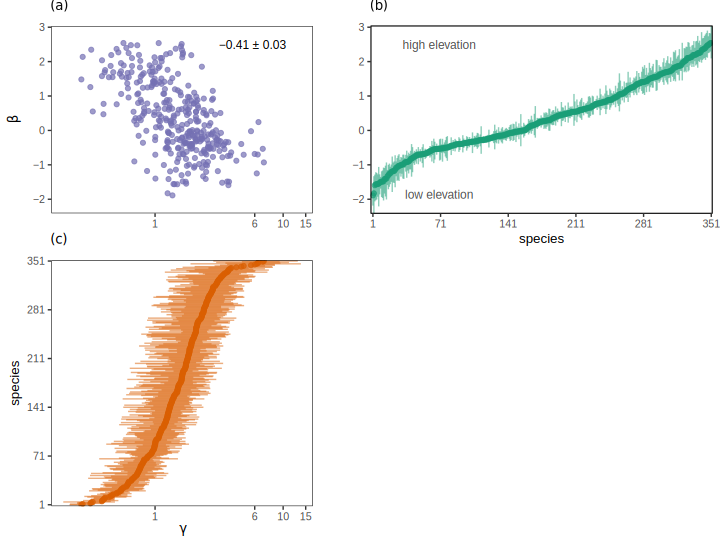
\includegraphics[width=0.9\textwidth]{figures/figure1-prime}
    	  \vspace{0.3cm}
	   \caption{Relationship between mean and variance of species' distributions. Posterior distributions for parameters $\beta_i$ and $\gamma_i$ from Eq.~(\ref{eq:baseline-response}) across species, and the relationship between them. Panel (a) describes the relationship between range size and elevation. Every dot represents the relationship between the mean values for the $\beta_i$ and $\gamma_i$ estimates of the different species. The value in the top-right corner of the plot displays the Pearson's correlation between these parameters calculated across samples of the posterior distributions. Panel (b) describes the $\beta_i$ posterior distribution estimated for all species. Panel (c) describes the $\gamma_i$ posterior distribution estimated for all species. In (b) and (c), the points represent the mean of the posterior distributions, and the corresponding lines characterize the 89\% confidence intervals.}
	   %7.5-5.5
      \label{fig:correlation}
\end{figure}

\begin{figure}[ht]
  \centering
    \vspace{0.5cm}
    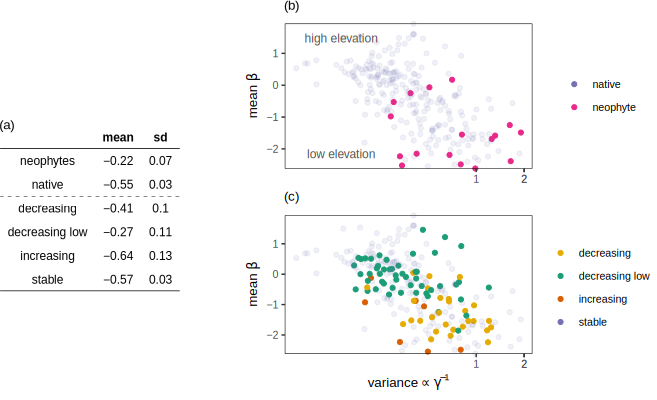
\includegraphics[width=0.9\textwidth]{figures/means-Rapopor}
    	  \vspace{0.3cm}
	   \caption{Universality of the relationship between mean and variance of species' distributions. Comparison between how different types of species are mapped in Fig.~\ref{fig:correlation}a. Panel (a) describes the correlation coefficient between $\beta_i$ and $\gamma_i$ for each type of species. Panel (b) shows the differences between neophytes and native species in the way these are distributed along the environmental gradient. Panel (c) shows the same differences for species that have decreased, decreased in low elevations, increase and remain stable over the last decades (see Supplementary Table 1 for further details). {\color{red} I might move this to the Supplementary Information.}}
	   %7.5-5.5
      \label{fig:universality}
\end{figure}

Maintaining the symmetry of species' distributions, we then allowed the kurtosis---or shape of the tails---of these to vary in different ways. To do so, we changed the response curve of our Bayesian model to follow a generalized error distribution (Eq.~\ref{eq:generalized-response}). A comparison of the WAIC values showed this non-linear regression to outperform the baseline model (Supplementary Fig.~XX)\footnote[2]{\label{note1} I am still waiting on the results for this (currently running in the cluster), and this is just my prior expectation based on what I've seen in some of the other models I've been working with.}. Studying the resulting posterior distributions, we found the parameter controlling for the kurtosis to be centred around $\nu_i \sim 2$, which corresponds to a distribution with a Gaussian shape (Fig.~\ref{fig:kurtosis-skewness}). However, such parameter estimates displayed a lot of variation across species, which might indicate that the shape of the tails of the distribution is species-specific (Supplementary Fig.~XX).

\begin{figure}[ht]
  \centering
    \vspace{0.5cm}
    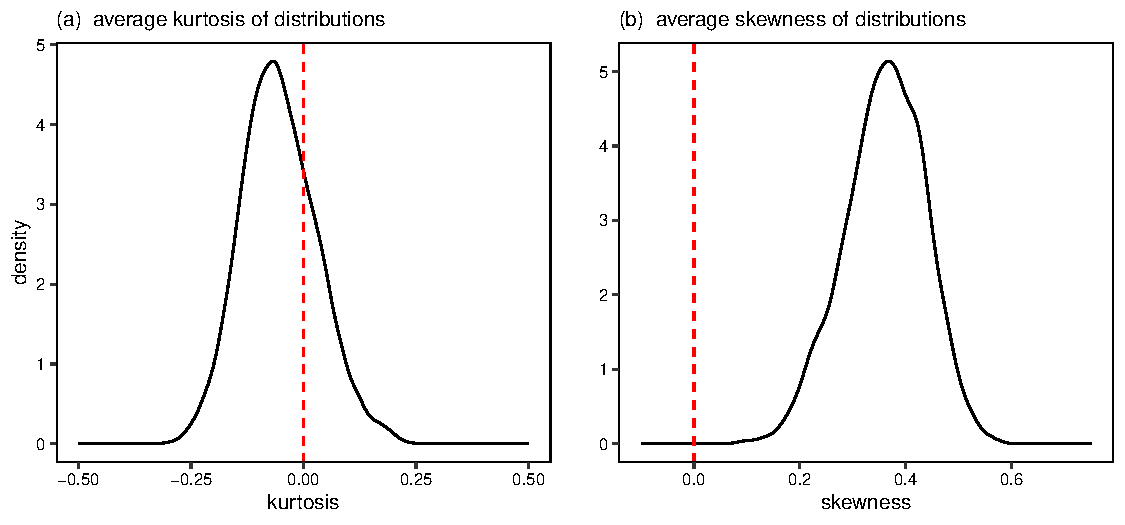
\includegraphics[width=0.8\textwidth]{figures/kurto-skew}
    	  \vspace{0.3cm}
	   \caption{Average kurtosis and skewness of species' distributions. Calculated using the posterior distributions of parameters $\hat{\nu}$ and $\hat{\lambda}$ from the models (see Supplementary Table XX), the two panels describe the average (a) kurtosis and (b) skewness of distributions, respectively. Panel (a) displays the results obtained by using a response curve that follows a generalized error distribution. Panel (b) displays the results obtained by using a response curve that follows a skewed normal distribution. In both case, the red dotted line indicates the conditions by which species are normally distributed along the environmental axis.}
      \label{fig:kurtosis-skewness}
\end{figure}

Next, we studied the skewness of species distributions using the skewed response curve in Eq.~(\ref{eq:skewed-response}). Based on the estimates for the WAIC values and Akaike weights, this model clearly outperformed the rest (Supplementary Fig.~XX), which sheds light on the naturally skewed nature of species' distributions. Studying the mean value of the skewness across species (i.e.~parameter $\hat{\lambda}$), we found that species' distributions showed steeper declines towards lower elevations (Fig.~\ref{fig:kurtosis-skewness}). Moreover, species' physiology seems to strongly shape this parameter, which suggest that distribution skewness is an intrinsic property of species (New Fig.~XX)\footref{note1}.
 
{\color{gray}
[Note: Reports on the hyperparameters describing the different covariance matrices missing at the moment. I think it's interesting, and I will certainly end up adding things here about this. I will also add a third figure showing how lambda varies with the corresponding variance-covariance matrix of species' environmental and physiological traits.]}

%The posterior distributions of the hyperparameters in Eq.~(\ref{eq:covariance-baseline}) revealed the value of this prior information on the different parameter estimates.  to understand the value of our prior information. 


%We then studied the level of information contained in physiological traits to explain the properties of distributions. Specifically, using Eq.~(\ref{eq:covariance-complex}), we accounted for both physiological and environmental traits in the variance-covariance structure for the mean and standard deviation of distributions. We information 
%As expected, the posterior distributions also showcase a positive relationship between... This is expected as ... Likewise, studying ... Following this, we added additional ... using Eq.~(\ref{eq:covariance-complex}). When studying plant... 
%Other interesting comparisons... The value of adding plant physiology as prior information for both the mean and standard deviation of the distributions. Informative in both case, specially for... Capturing some of bla bla bla.

%Then, we stud the tails of distributions by modifying the baseline model to account for different properties. Kurtois. Studying the parameter... Similar values were found for binary data and the model did not outperform the baseline model

% Next we studied the skewness of distributions, outpreforming the other models. When studying the parameter, we found that the mean skewness of species distributions declined... Hypothesis! When accounting for plant physiology as priors for the skewness of distribution, we found this to be ... Figure and Hypothesis. The model also showcased the Rapopor's hypothesis...

%%%%%%%%%%%%%%%%%%%%%%%%%%%%%%%%%%%%%%%%%%%%%%%%%%%%%%
%%       DISCUSSION
%%%%%%%%%%%%%%%%%%%%%%%%%%%%%%%%%%%%%%%%%%%%%%%%%%%%%%
\section*{Discussion}
%In this work, we used non-linear response curves to model the distribution of species across an environmental gradient. First, we used a baseline model that considered species to present bell-shaped distributions. Studying the parameter estimates across species, we were able to showcase how species follow the Rapopor's rule along an elevation gradient. Second, we used several...
Structure of the discussion section:
\begin{enumerate}
\item Summary of results.
\item Proper test of Rapopor's hypothesis. Different species follow different biogeographical patterns.
\item Proper test of skewed towards high altitude. Is species' physiology informative to explain the pattern? 
\item What is the true shape of species' distributions? These display heavy-tail and skewed distributions. 
\item Future directions. Missing bimodal curves. Using this information to understand where jSDMs estimate interactions between species. Further test of the ability of traits to predict those parameter estimates.
\end{enumerate}
% Summary of results
% Proper test of Rapopor's hypothesis. Different species follow different biogeographical patterns.
% Proper test of skewed towards high altitude. Is species' physiology informative to explain the pattern? 
% What is the true shape of distributions? Missing bimodal curves
% 

%%%%%%%%%%%%%%%%%%
%%% Model runs
%%%%%%%%%%%%%%%%%%
% Finish categorical 1d for both skewed and normal (2 weeks)
% Test for heavy tails 1 binomial and categorical (0.5 week)
% Test for heavy tails 2 binomial and categorical (0.5 week)
% Categorical 1d for heavy tails 1 (1 weeks)
% Categorical 1d for heavy tails 2 (1 weeks)
% Binomial 1d for heavy tails 1 (0.7 weeks)
% Binomial 1d for heavy tails 2 (0.7 weeks)
% Binomial 1d for skewed (0.7 weeks)
% Binomial 1d normal two covariances (1 week)
% Categorical 1d for skewed with physiology in lambda (1 week)
% Additional tests for Binomial 1d skewed and normal (1 week)

% With both heavy-tails ~ 10 weeks
% With only one heavy-tail ~ 8 weeks

\clearpage
\bibliography{references2}

\end{document}
